\documentclass[10pt]{article}
\usepackage[total={170mm,230mm}]{geometry}

\usepackage{cmap}
\usepackage{hyperref}
\usepackage[utf8]{inputenc}
\usepackage[T2A]{fontenc}
\usepackage[russian]{babel}

\usepackage{graphicx}
\usepackage{xcolor}
\usepackage{amssymb}
\usepackage{amsfonts}
\usepackage{amsmath}
\usepackage{amsthm}
\usepackage{physics}
\usepackage{wrapfig}
\usepackage{cancel}
\usepackage{pdfpages}
\usepackage{hyperref}
\usepackage{caption}
\usepackage{subcaption}
% \usepackage{bibtex}

\title{Домашнее задание №4. Метод подбора постоянной связи}
\author{Александр Козлов}
\date{\today}

\begin{document}

\maketitle

\section*{Формулировка задания}

Дан гамильтониан одномерной квантово-механической системы с потенциалом в виде гауссовой ямы
\begin{equation}
    H = - \dv[2]{}{x} + V_0\, e^{-x^2},
\end{equation}
где $V_0 < 0$. Требуется с помощью метода подгонки константы связи:
\begin{enumerate}
 \item найти основное состояние;
 \item[2*.] найти возбужденные состояния.
\end{enumerate}


\section{Дискретизация задачи}

Рассматриваемое уравнение Шрёдингера (УШ) имеет вид
\begin{equation}
    -\dv[2]{\psi}{x} + V_0\, e^{-x^2}\, \psi  = E\, \psi
    \label{eq:SE}
\end{equation}
или
\begin{equation}
    \dv[2]{\psi}{x}  + (E - V_0\, e^{-x^2})\, \psi  = 0.
\end{equation}
Стоит заметить, что такое уравнение соответствует обычному одномерному УШ при $\hbar=1$ и $m=1/2$.

Прежде всего зададим равномерную сетку
\begin{equation}
    x_0 = -R,\; x_1 = x_0 + \delta,\; x_2 = x_0 + 2\delta,\; \ldots,\; x_k = x_0 + k\delta,\; \ldots,\; x_M = x_0 + M \delta = R
\end{equation}
с шагом $\delta = 2R/M$, где $M$~---~целое положительное число, а $R$~---~положительное действительное число. Будем пользоваться численной аппроксимацией второй производной
\begin{equation}
    \dv[2]{\psi}{x}(x_k) = \dfrac{\psi(x_{k+1}) - 2\psi(x_{k}) + \psi(x_{k-1})}{\delta^2} + O(\delta^2),\quad k = \overline{1,M-1}
\end{equation}
и сводить уравнение \eqref{eq:SE} к задаче диагонализации трёхдиагональной матрицы.

Перед тем, как писать явный вид такой матрицы, необходимо поговорить о том, как будут задаваться граничные условия. Ясно, что волновые функции состояний дискретного спектра будут экспоненциально затухать при больших по абсолютному значению $x$. Это обстоятельство может быть численно учтено различными вариантами, однако, остановимся на варианте, при котором полагается $\psi(x_0) = \psi(x_M) = 0$. Тогда численное приближение УШ для $k=1$ примет вид
\begin{equation}
    -\dfrac{\psi(x_{2}) - 2\psi(x_{1})}{\delta^2} + V(x_1)\,\psi(x_1) = E\psi(x_1).
\end{equation}
Для $k=M-1$ получаем аналогичное уравнение
\begin{equation}
    -\dfrac{-2\psi(x_{M-1})+\psi(x_{M-2}) }{\delta^2} + V(x_{M-1})\,\psi(x_{M-1}) = E\psi(x_{M-1}).
\end{equation}
А для всех остальных $k$ имеем уравнение
\begin{equation}
    -\dfrac{\psi(x_{k+1}) - 2\psi(x_{k}) + \psi(x_{k-1})}{\delta^2} + V(x_k)\,\psi(x_k) = E\psi(x_k).
\end{equation}
В матричном виде задача записывается так:
\begin{equation}
\begin{split}
    &\begin{pmatrix}
        2\delta^{-2}+V(x_1)& -\delta^{-2}\\
        -\delta^{-2}& 2\delta^{-2}+V(x_2)& -\delta^{-2}\\
        % & -\delta^{-2}& 2\delta^{-2}+V_0\,e^{-x_3^2}& -\delta^{-2}\\
        & & & \ddots&\\
        & & & & -\delta^{-2}& 2\delta^{-2}+V(x_{M-2})& -\delta^{-2}\\
        & & & & & -\delta^{-2}& 2\delta^{-2}+V(x_{M-1})
    \end{pmatrix}
    \begin{pmatrix}
        \psi(x_1)\\
        \psi(x_2)\\
        \vdots\\
        \psi(x_{M-2})\\
        \psi(x_{M-1})
    \end{pmatrix}\\
    &=E
    \begin{pmatrix}
        \psi(x_1)\\
        \psi(x_2)\\
        \vdots\\
        \psi(x_{M-2})\\
        \psi(x_{M-1})
    \end{pmatrix}.
\end{split}
\end{equation}

\section{Метод подбора постоянной связи}

Задачу требуется решить методом побора постоянной связи. Рассмотрим главные идеи такого метода. Во-первых, введём \emph{резольвенту} для дискретизованного оператора кинетической энергии  $\hat T$ (шляпки над символами означают дискретизованный оператор)
\begin{equation}
 \hat R(z) = \qty(\hat T - z \hat I)^{-1},
\end{equation}
где $z$~---~любое число. Тогда нетрудно показать, что задача на отыскание спектра гамильтониана эквивалентна задаче на отыскание таких величин $z$, при которых собственные числа $\lambda(z)$ задачи
\begin{equation}
 - \hat R(z)\, \hat V \phi = \lambda(z) \phi
\end{equation}
равны 1, при этом найденные величины $z$ и составят искомый спектр энергий $E$.

\section{Метод простой итерации для нахождения основного состояния}

Введём обозначение $ \hat{\mathcal{L}}(z) = - \hat R(z)\, \hat V$. Собственные значения оператора $\hat{\mathcal{L}}(z)$ дают семейство ветвей $\lambda_k(z)$. Чтобы найти спектр гамильтониана нужно решить уравнения $\lambda_k(z)=1$ для каждого $k$, спектр составят найденные корни.

Для нахождения основного состояния можно воспользоваться методом простой итерации, так как основному состоянию отвечает верхняя ветка  $\lambda_0(z)$. То есть идея проста. Находим для какого-то набора значений ${z_i} \in (V_0,\; 0.0)$ наибольшие по абсолютной величине собственные значения операторов $\hat{\mathcal{L}}(z_i)$ $\lambda_0(z_i)$ методом простой итерации, интерполируем значения $\lambda_0(z_i)$ кубическими сплайнами и решаем уравнение $\lambda_0(z)=1$.

Такой подход позволяет получить достаточно точно величины энергий основных состояний. На Рис. \ref{fig:-1.0_l0} и на Рис. \ref{fig:-5.0_l0} показаны получившиеся ветки $\lambda_0(z)$ для $V_0 = -1.0$ и $V_0=-5.0$ соответсвенно.
\begin{figure}[htbp]
 \centering
 \begin{subfigure}[b]{0.49\textwidth}
    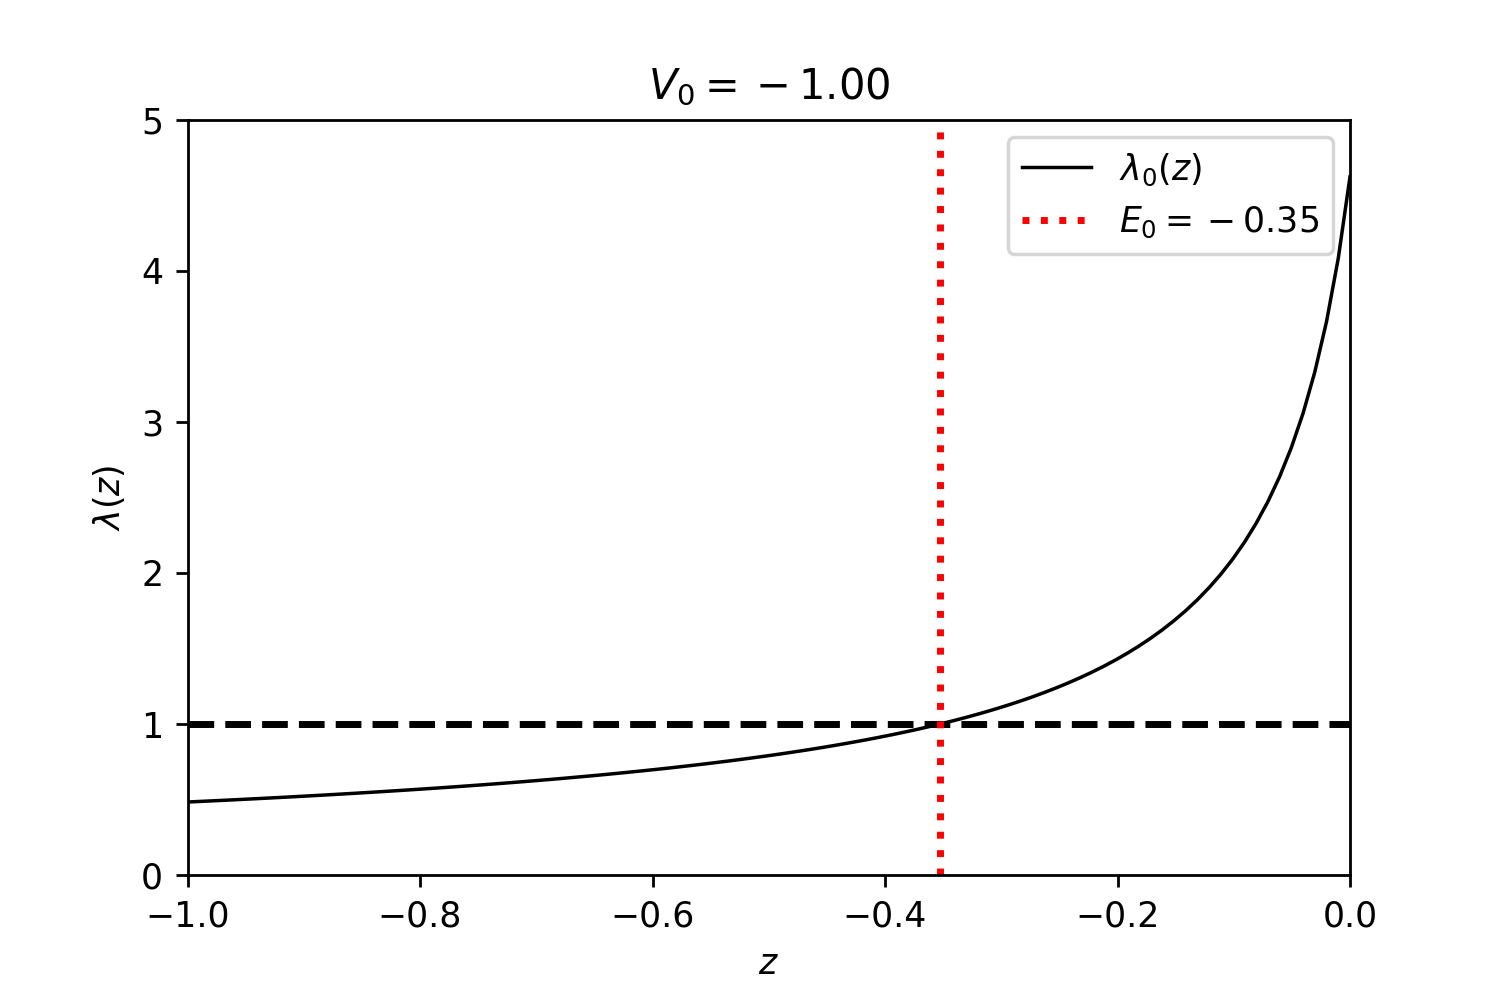
\includegraphics[width=\textwidth]{../figures/-1.0_l0}
    \caption{Верхняя ветвь $\lambda_0(z)$ при $M=1000$ и $R=6.0$ для случая $\abs{V_0}=1$. Вертикальной линией отмечено получившееся решение.}
    \label{fig:-1.0_l0}
\end{subfigure}
\hfill
\begin{subfigure}[b]{0.49\textwidth}
    \centering
    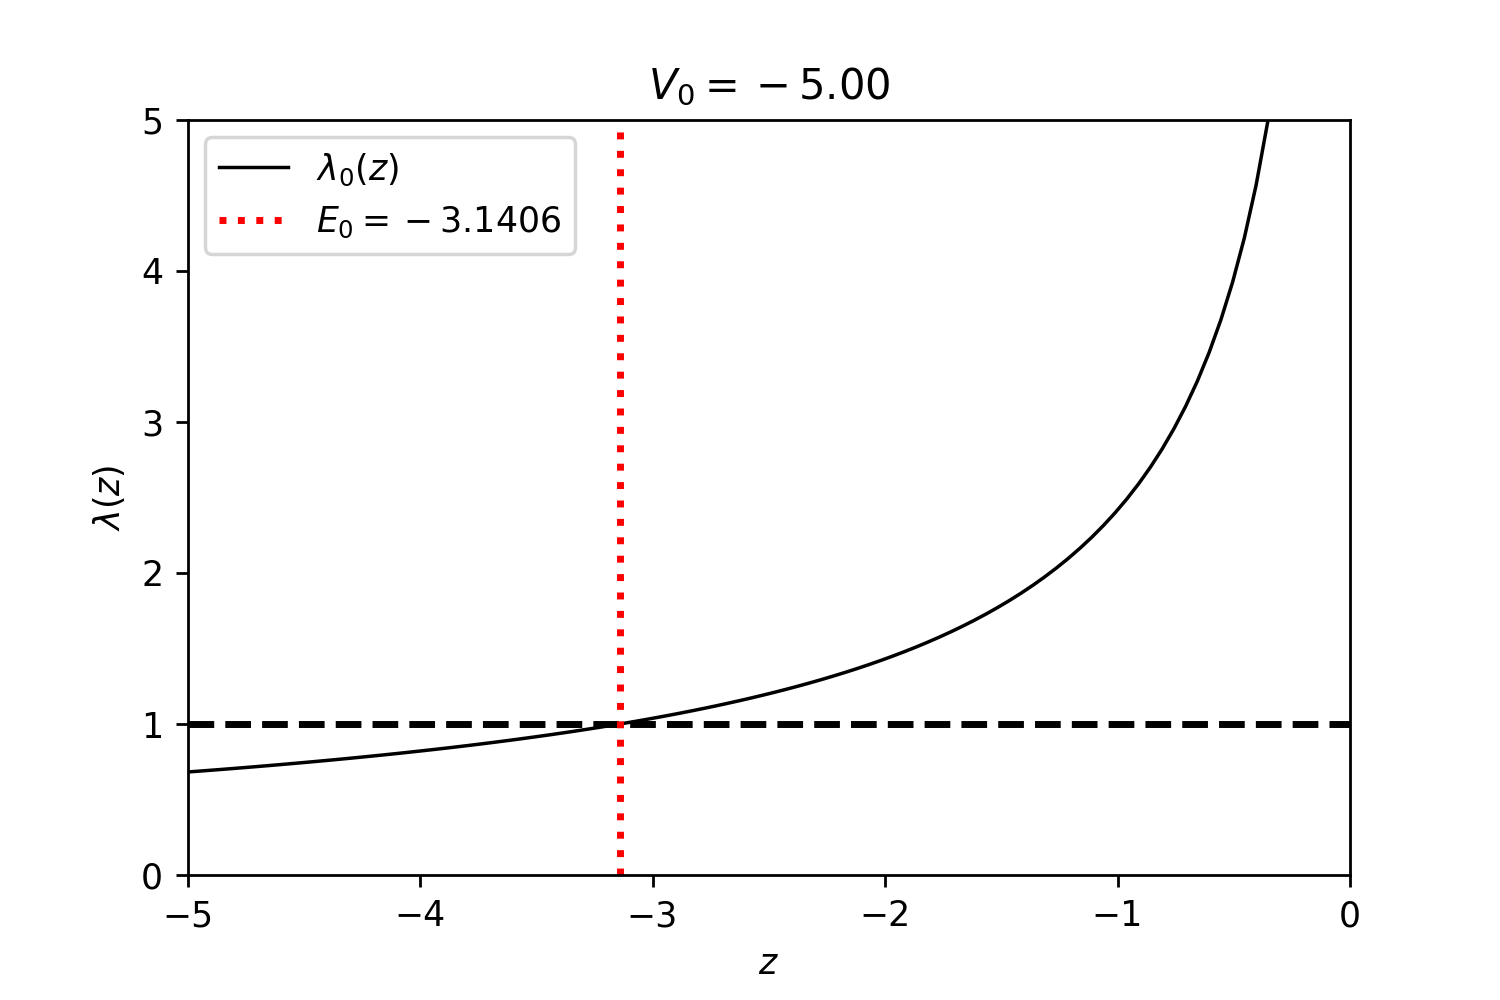
\includegraphics[width=\textwidth]{../figures/-5.0_l0}
    \caption{Верхняя ветвь $\lambda_0(z)$ при $M=1000$ и $R=6.0$ для случая $\abs{V_0}=5$. Вертикальной линией отмечено получившееся решение.}
    \label{fig:-5.0_l0}
\end{subfigure}
\end{figure}




\section{Метод итераций Арнольди для отыскания основных и возбужденных состояний}

Для отыскания большего числа ветвей можно применить метод итераций Арнольди, который основан на том, чтобы использовать подпространство Крылова
$$
K_n(z_i) = \qty[\phi_0,\; \hat{\mathcal{L}}(z_i)\phi_0,\; \ldots,\; \hat{\mathcal{L}}^{n-1}(z_i)\phi_0],
$$
получающееся в результате использования метода простой итерации с начальной волвой функцией $\phi_0$, для постоения в нём ортогонального базиса, которое и даст первые $n$ собственных значений опертора $\hat{\mathcal{L}}(z_i)$.

На Рис. \ref{fig:-1.0_l5} и на Рис. \ref{fig:-5.0_l5} показаны первые пять получившихся ветвей $\qty{\lambda_k(z)}_{k=0}^4$ для $V_0 = -1.0$ и $V_0=-5.0$ соответсвенно.
\begin{figure}[htbp]
 \centering
 \begin{subfigure}[b]{0.49\textwidth}
    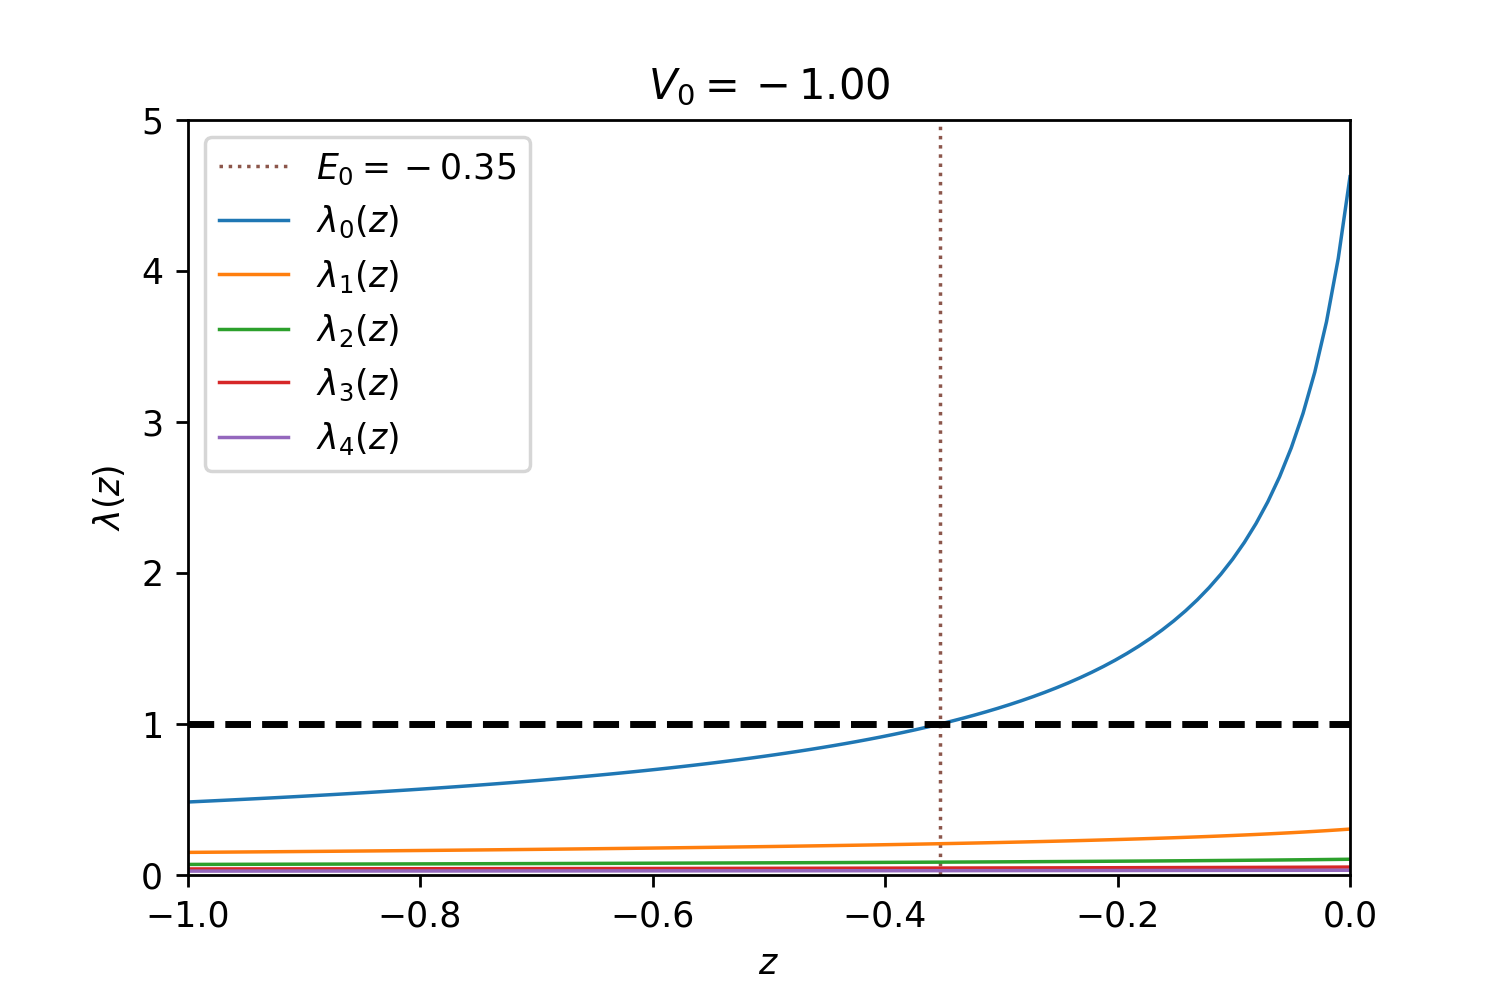
\includegraphics[width=\textwidth]{../figures/-1.0_l5}
    \caption{Первые пять ветвей $\qty{\lambda_k(z)}_{k=0}^4$ при $M=1000$ и $R=6.0$ для случая $\abs{V_0}=1$. Вертикальными линиями отмечены получившиеся решения.}
    \label{fig:-1.0_l5}
\end{subfigure}
\hfill
 \begin{subfigure}[b]{0.49\textwidth}
    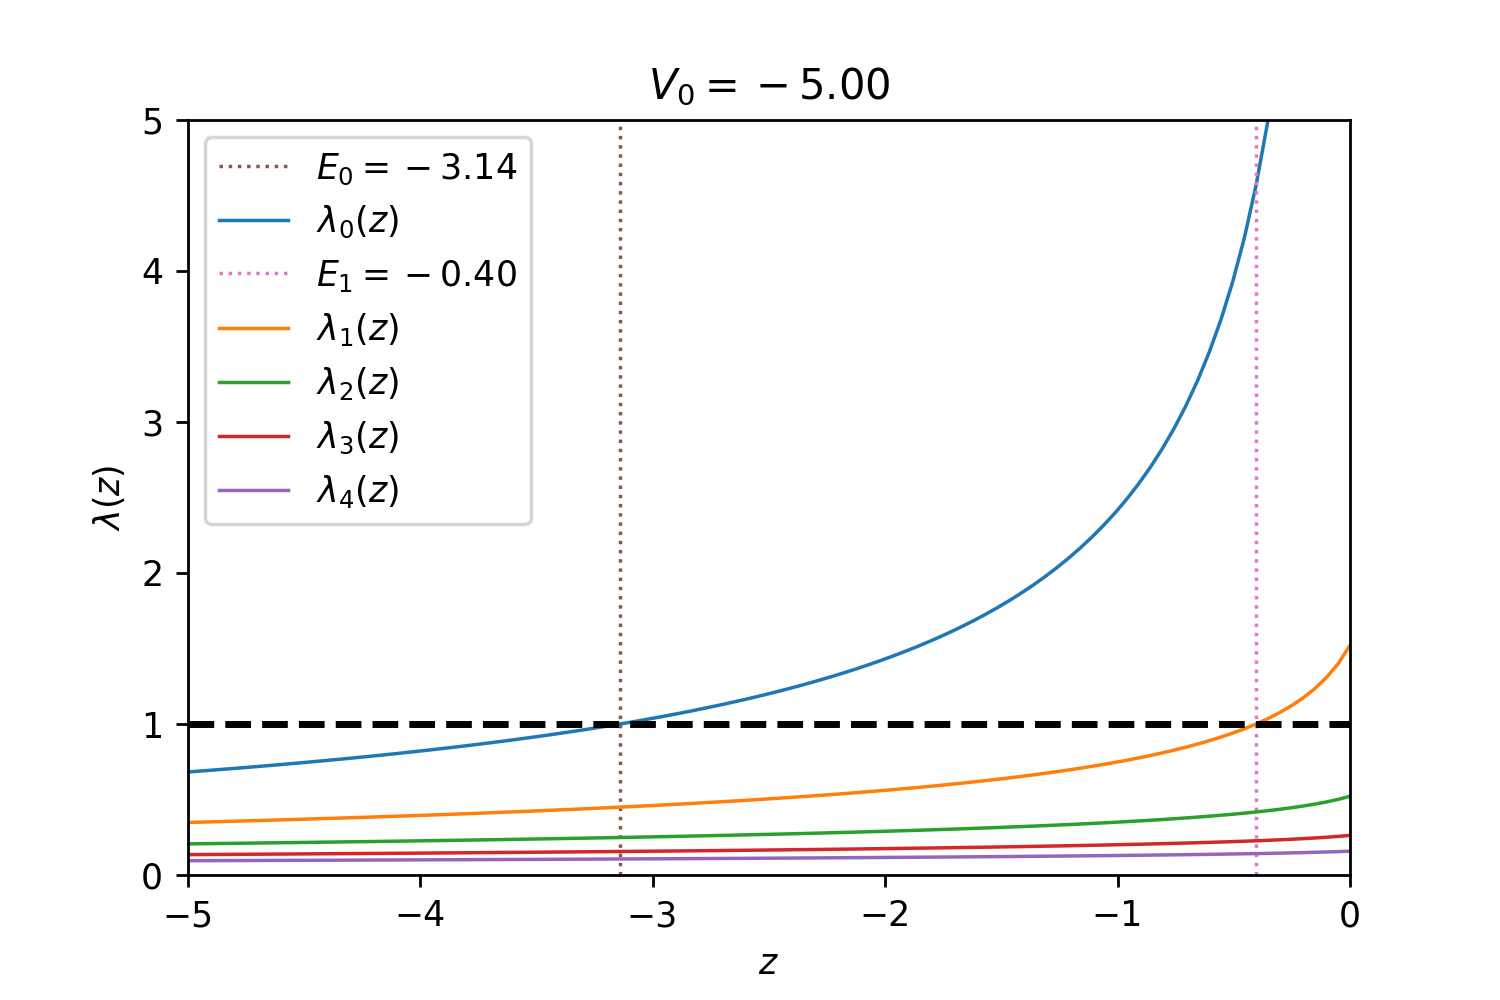
\includegraphics[width=\textwidth]{../figures/-5.0_l5}
    \caption{Первые пять ветвей $\qty{\lambda_k(z)}_{k=0}^4$ при $M=1000$ и $R=6.0$ для случая $\abs{V_0}=5$. Вертикальными линиями отмечены получившиеся решения.}
    \label{fig:-5.0_l5}
\end{subfigure}
\end{figure}

\end{document}
